\documentclass[a4paper,12pt]{article}
\RequirePackage[l2tabu, orthodox]{nag}
\usepackage{setspace}
\usepackage{amsfonts}
\usepackage{amsmath}
\usepackage{booktabs}
\usepackage{multirow}
\usepackage{amsmath}
\usepackage{float}
\usepackage{graphicx}
\restylefloat{table}
\usepackage{braket}
%Enable fr support
\usepackage[utf8]{inputenc} 
\usepackage[T1]{fontenc} 
\usepackage{lmodern} % load a font with all the characters
\usepackage{listings}
\usepackage{color}

\definecolor{dkgreen}{rgb}{0,0.6,0}
\definecolor{gray}{rgb}{0.5,0.5,0.5}
\definecolor{mauve}{rgb}{0.58,0,0.82}

\lstset{frame=tb,
	language=Java,
	aboveskip=3mm,
	belowskip=3mm,
	showstringspaces=false,
	columns=flexible,
	basicstyle={\small\ttfamily},
	numbers=none,
	numberstyle=\tiny\color{gray},
	keywordstyle=\color{blue},
	commentstyle=\color{dkgreen},
	stringstyle=\color{mauve},
	breaklines=true,
	breakatwhitespace=true,
	tabsize=3
}
%Assign document variables
\date{\today}
\title{Travail \#6}
\author{tmp}
\newcommand{\Author}{Kevin Belisle}
\newcommand{\Authorr}{Olivier Bélec}
\newcommand{\MatriculeAuthor}{20018469}
\newcommand{\MatriculeAuthorr}{00000000}
\newcommand{\Teacher}{Abdelhakim Hafid}
\newcommand{\ClassNum}{IFT-3325}
\newcommand{\ClassName}{Téléinformatique}
\newcommand{\DateMMMMYYYY}{Novembre 2018}
\newcommand{\tab}[1]{\hspace{.05\textwidth}\rlap{#1}}
\makeatletter
\makeatother
\makeatletter
%Custom Header & Footer
\usepackage{fancyhdr}
\pagestyle{fancy}
\fancyhf{}
\fancyhead[L]{\@title}
\fancyhead[R]{\thepage}
\fancyfoot[L]{Kevin Belisle}
\fancyfoot[R]{\DateMMMMYYYY}
\renewcommand{\footrulewidth}{0.4pt}% default is 0pt

\begin{document}
	\begin{titlepage} 
		\begin{center}
			\textsc{\normalsize Université de Montréal}\\[3cm]
			 
			\textsc{\LARGE \@title}\\[2.5cm]
			
			\textsc{\small Par}\\[0.25cm]
			\textsc{\LARGE \Author}\\[0.25cm]
			\textsc{\normalsize (\MatriculeAuthor)}\\[0.25cm]
			\textsc{\LARGE \Authorr}\\[0.25cm]
			\textsc{\normalsize (\MatriculeAuthorr)}\\[2.25cm]
			
			\textsc{\normalsize Baccalauréat en informatique}\\
			\textsc{\normalsize Faculté des arts et des sciences}\\[2.5cm]
			
			\textsc{\small Travail présenté à \Teacher}\\
			\textsc{\small Dans le cadre du cours \ClassNum}\\
			\textsc{\small \ClassName}\\[2.75cm]
			
			\textsc{\normalsize \DateMMMMYYYY}\\[1.5cm]
		\end{center}
	\end{titlepage}
	\begin{spacing}{1}
	\section*{Diagramme de classe}
	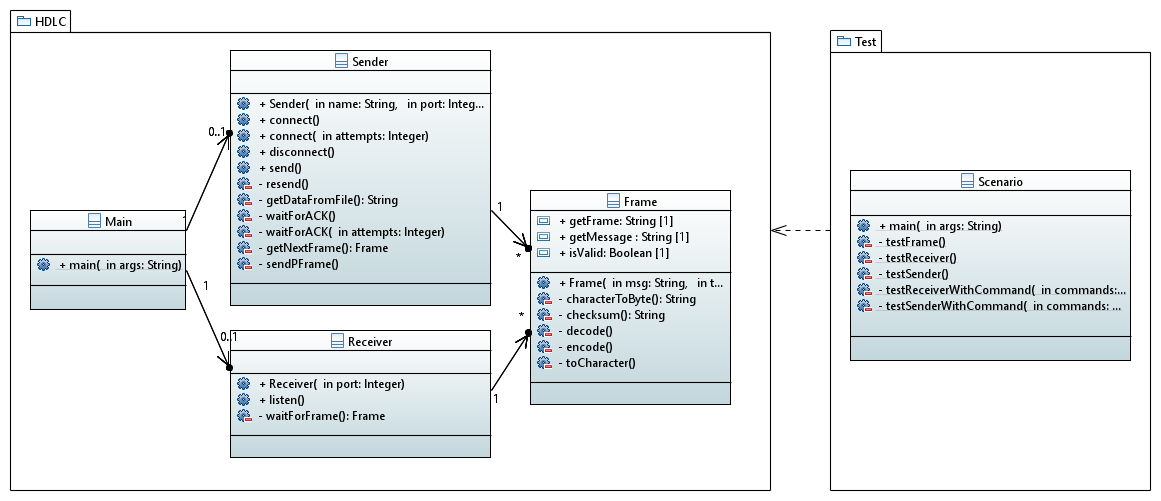
\includegraphics[scale=0.4]{ClassDiagram.png}
	\section*{Description des classes}
	\subsection*{Sender}
	\subsubsection*{Constantes}
	\begin{lstlisting}
	private final static int DATA_SIZE_LIMIT = 100; 
	private final static int MAX_BUFFER_WINDOW_SIZE = 8;
	private final static int MAX_FRAME_COUNT = 7; /*2^3-1 = 7*/
	private final static int MAX_WAIT_TIME = 3000;
	private final static int MAX_ATTEMPT = 30;
	private final static int ACK_FRAME_SIZE = 48;
	\end{lstlisting}
	\textbf{DATA\_SIZE\_LIMIT} : Le nombre de caractère que nous envoyions par trame. Elle sert à simuler un maximum sur le data pour chaque trame.\\\\
	\textbf{MAX\_BUFFER\_WINDOW\_SIZE} : La grandeur maximum du buffer pour les trames ($2^3$, car nous utilisons 3 bits pour numéroter les trames). \\\\
	\textbf{MAX\_FRAME\_COUNT} : Le nombre maximum de trame en mémoire à un moment donné ($2^3-1$ pour Go-Back-N).\\\\
	\textbf{MAX\_WAIT\_TIME} : Le temps maximum d'attente pour le temporisateur (3s pour ce TP).\\\\
	\textbf{MAX\_ATTEMPT} : Le nombre maximum d'essai avant de conclure que la connexion avec le serveur est perdu.\\\\
	\textbf{ACK\_FRAME\_SIZE} : la taille des trames de réponse (Elles sont tout le temps de taille 6 octets pour ce TP, donc 6octets*8bits/octets = 48 bits).
	\subsubsection*{Attributs}
	\begin{lstlisting}
	Socket s;
	DataInputStream in;
	DataOutputStream out;
	BufferedReader file;
	Frame[] frameBuffer = new Frame[MAX_BUFFER_WINDOW_SIZE];
	int nextEmpty = 0;
	int lastACK = MAX_BUFFER_WINDOW_SIZE - 1;
	int frameCount = 0;
	boolean sendingData = false;
	\end{lstlisting}
	Nous gardons en mémoire les éléments suivants en ordre de haut en bas : le socket (s), le flux d'entrée du socket (in), le flux de sortie du socket (out), le flux du fichier(file), le buffer pour les trames(frameBuffer), l'index de la prochaine case du tableau qui est vide(nextEmpty), le numéro de la dernière trame qui a été acquiescée(lastACK), le nombre de frame dans le buffer (frameCount) et si nous envoyons ou non des données (sendingData).
	\subsubsection*{Constructeur}
	\begin{lstlisting}
	public Sender(String name, int port, String fileName)
	\end{lstlisting}
	Unique Construteur qui initialise le socket vers le \textit{serveur} sur le \textit{port}, ouvre le fichier et garde en mémoire le flux d'entrée, de sortie et du fichier.
	\subsubsection*{Méthodes}
	\begin{lstlisting}
	private void waitForACK() /*waitForACK(0)*/
	private void waitForACK(int attempts) 
	\end{lstlisting}
	Attend la prochaine trame de réponse du serveur et la traite.
	\begin{lstlisting}
	public void connect() /*connect(0)*/
	private void connect(int attempt)
	\end{lstlisting}
	Envoie la trame de demande de connexion au serveur et attends la trame de réponse.
	\begin{lstlisting}
	public void disconnect()
	\end{lstlisting}
	Envoie la trame de connexion et relâche toutes les ressources (socket et flux).
	\begin{lstlisting}
	private String getDataFromFile()
	\end{lstlisting}
	Lit du flux du ficher le nombre de caractère maximal spécifié par la constante DATA\_SIZE\_LIMIT
	\begin{lstlisting}
	public void send()
	\end{lstlisting}
	Commencer l'envoie des données vers le serveur.
	\begin{lstlisting}
	private void resend()
	\end{lstlisting}
	Réenvoie toutes les trames qui sont en mémoire.
	\begin{lstlisting}
	private Frame getNextFrame()
	\end{lstlisting}
	Bloque et attends (si nécesaire), lit du flux d'entrée la trame de réponse provenant du serveur et retourne la trame pour futur traitement.
	\begin{lstlisting}
	private void sendPFrame(int attempts)
	\end{lstlisting}
	Envoie une trame P-bit au serveur.
	\subsection*{Receiver}
	\subsubsection*{Attributs}
	\begin{lstlisting}
	Frame lastMsg;
	int next;
	long timer;
	String txt="";
	/*socket*/
	ServerSocket server;
	Socket socket;
	DataInputStream input;
	DataOutputStream output;
	\end{lstlisting}
	Nous gardons en mémoire les attributs suivants en order de haut en bas: la trame du dernier message (lastMsg), le prochain numéro de trame (next), le temps courant (timer), le data reçu du sender (txt), le serveur de socket (server), le socket (socket), le flux d'entrée du socket (input) et le flux de sortie du socket (output).
	\subsubsection*{Constructeur}
	\begin{lstlisting}
	public Receiver(int port)
	\end{lstlisting}
	Instancie le Receiver, créer le serveur pour les sockets sur le port spécifié, instancie un socket sur le serveur et garde en mémoire les flux d'entrée et de sortie du socket.
	\subsubsection*{Méthodes}
	\begin{lstlisting}
	public void listen()
	\end{lstlisting}
	Écoute sur le socket pour des trames, sauvegarde le data des trames et envoie les trames de réponse appropriés
	\begin{lstlisting}
	private Frame waitForFrame()
	\end{lstlisting}
	Bloque et attends (si nécessaire) pour des trames du Sender et les retourne pour un futur traitement.
	\subsection*{Frame}
	\subsubsection*{Attributs}
	\begin{lstlisting}
	private boolean valid;
	private String message,encoded;	
	public String getMessage()
	public String getFrame() 
	public Boolean isValid()
	\end{lstlisting}
	Nous gardons en mémoire si la trame est valide ou non (valid et isValid()), le message décodé (message, getMessage()) et le message encodé (encoded, getFrame()).
	\subsubsection*{Constructeur}
	\begin{lstlisting}
	public Frame(String msg,boolean toBeEncoded)
	\end{lstlisting}
	Instancie une trame. En fonction de (toBeEncoded), nous encoderons la trame et nous la décoderons sinon.
	\subsubsection*{Méthodes}
	\begin{lstlisting}
	private void encode()
	\end{lstlisting}
	Encode le message de la trame, fait du bit-stuffing et calcule le CRC.
	\begin{lstlisting}
	private void decode()
	\end{lstlisting}
	Décode le message encodé de la trame, défait le bit-stuffing et vérifie le contenu selon le CRC.
	\begin{lstlisting}
	private String checksum(String msg)
	\end{lstlisting}
	Calcule le CRC à partir du contenu de la trame.
	\begin{lstlisting}
	private String characterToByte()
	\end{lstlisting}
	Transforme une chaîne de caractères en octets.
	\begin{lstlisting}
	public void toCharacter()
	\end{lstlisting}
	Transforme des octets en caractères.
	\end{spacing}
	\subsection*{Main}
	Point d'entrée de l'application, valide les arguments d'entrée et créer le Sender ou Receiver selon les arguments d'entrée
\end{document}